\scanpage{150}
{\ttfamily\unsure{ACCOUNT NUMBER}\quad\unsure{**********}\quad DATE = 82.231\quad TIME = 8.51.16\quad SYSTEM 370/081 E333\quad VS2 \unsure{03.8G|03.86}\\
JOBNAME= CRAY2\quad NUMBER=231J002\unsure{5|S}CNU\quad CPU TOTAL = 1\quad RATE = 0, 1}
\diagram{{\tiny\begin{tabular}{cc|cc|cccccccccc|cc|c}
\multicolumn{2}{c|}{STEP}&\multicolumn{2}{c|}{TIME}&\multicolumn{10}{c|}{NUMBER OF EXCPS}&\multicolumn{2}{c|}{BYTES}&\\
NO&CORE&TIO&TCPU&3330&3330-1&3340&3350&2250&\unsure{T/7TRK}&\unsure{T/9-16}&T/6250&SPOOL&VIO&SYSIN&SYSOUT&C.U\\\hline
1&8&\unsure{4}&1&0&0&0&0&0&0&0&0&1&0&0&0000288&105\\\hline
\multicolumn{2}{c|}{TOTALS}&\unsure{4}&1&0&0&0&0&0&0&0&0&1&0&0&0000288&105
\end{tabular}}}
\diagram{{\tiny\begin{tabular}{ccccc|cc|cccc|cccc|c|c}
\multicolumn{5}{c|}{STEP}&\multicolumn{2}{c|}{PAGING}&\multicolumn{4}{c|}{SWAP}&\multicolumn{4}{c|}{VIO}&CORE&SETUP TIME\\
NO&NAME&P.G.M&C.C.U&SRB&IN&OUT&N&OUT&P.IN&P.OUT&TOT&TOP&DU&OM&TU&TM.ELAPS\\\hline
1&&\unsure{IEFBR14|TEFBR14}&105&0&0&0&0&0&0&0&6064&200&0&0&0&0\quad0\\\hline
\multicolumn{3}{c}{TOTALS}&\unsure{300}&0&0&0&0&0&0&0&\unsure{0}&\unsure{0}&0&0&0&0\quad0
\end{tabular}}}
{\ttfamily\unsure{RESOURCES ESTIMATED}\quad ( SYSOUT = \unsure{0130000|0120000}\quad EXCP = 1000\quad TIME = 6\quad REGION = 150K )\quad GIVING CLASS/PRIO = 1/ 6\\
RESOURCES USED\quad ( \unsure{SYSOUT = 0000288}\quad EXCP = 0\quad TIME = 1\quad REGION = 8K )\quad GIVING CLASS/PRIO = A/14\\
\unsure{\$HASP399} ENDED}
\figure{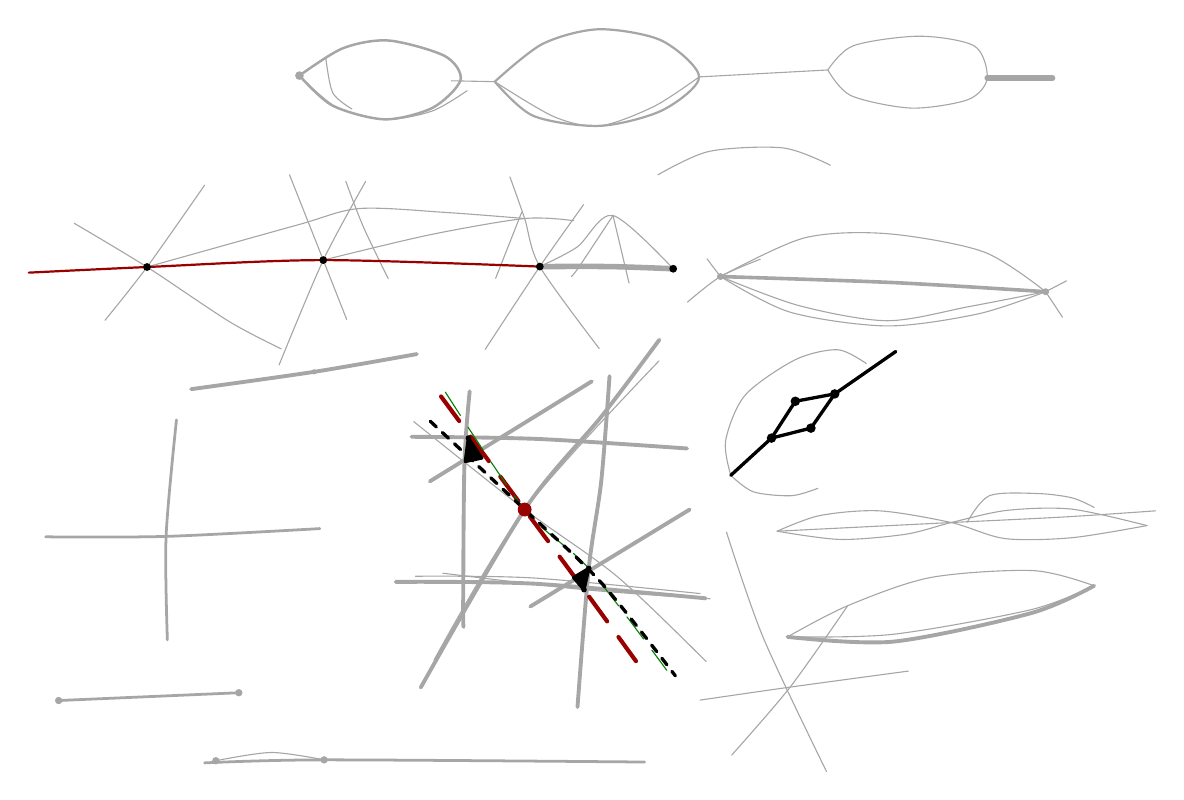
\begin{tikzpicture}[x=.55cm,y=-.55cm,line cap=round,line join=round,g/.style={olive!80!yellow,line width=1.7pt},r/.style={orange!80!brown,line width=1.8pt},w/.style={red!60!black,line width=1.5pt},b/.style={blue!60!black,line width=1.4pt},p/.style={gray!70,thin},k/.style={black,line width=1.2pt},every node/.style={font=\scriptsize}]
% Upper chain of three pencil loops.
\draw[p,line width=.9pt] plot[smooth] coordinates {(9.72,4.21) (10.72,3.58) (11.78,3.4) (13.08,3.76) (13.44,4.31) (12.8,4.95) (11.69,5.22) (10.48,4.9) (9.72,4.21)};
\draw[p] plot[smooth] coordinates {(9.72,4.21) (10.56,4.93) (11.69,5.22) (12.78,5.03) (13.59,4.56)};
\draw[p] plot[smooth] coordinates {(10.33,3.82) (10.49,4.61) (10.93,4.98)};
\draw[p] plot[smooth] coordinates {(13.23,4.33) (14.23,4.35)};
\draw[p,line width=.8pt] plot[smooth] coordinates {(14.23,4.35) (15.33,3.48) (16.63,3.14) (18.08,3.4) (18.95,4.24) (18.1,5.01) (16.66,5.37) (15.12,5.14) (14.23,4.35)};
\draw[p] plot[smooth] coordinates {(14.23,4.35) (15.6,5.16) (16.66,5.37) (17.91,4.92) (18.95,4.24)};
\draw[p] plot[smooth] coordinates {(18.95,4.24) (21.92,4.08)};
\draw[p] plot[smooth] coordinates {(18.0,6.5) (19.18,5.96) (20.89,5.88) (21.98,6.28)};
\draw[p] plot[smooth] coordinates {(21.92,4.08) (22.51,3.52) (24.04,3.3) (25.31,3.53) (25.6,4.27) (25.17,4.76) (23.85,4.96) (22.45,4.67) (21.92,4.08)};
\draw[p,line width=2pt] plot[smooth] coordinates {(25.6,4.27) (27.11,4.27)};
\fill[p] (9.72,4.21) circle (.1);
% Horizontal line with three marked crossings and pencil detours.
\draw[p] plot[smooth] coordinates {(4.52,7.62) (6.2,8.63) (8.1,9.89) (9.3,10.52)};
\draw[p] plot[smooth] coordinates {(7.53,6.74) (6.2,8.63) (5.23,9.86)};
\draw[p] plot[smooth] coordinates {(9.49,6.5) (10.27,8.47) (10.81,9.84)};
\draw[p] plot[smooth] coordinates {(11.25,6.65) (10.27,8.47) (9.25,10.89)};
\draw[p] plot[smooth] coordinates {(10.79,6.65) (11.19,7.69) (11.77,8.9)};
\draw[p] plot[smooth] coordinates {(14.58,6.55) (14.92,7.51) (15.27,8.62) (16.64,10.51)};
\draw[p] plot[smooth] coordinates {(16.28,7.19) (15.27,8.62) (14.01,10.53)};
\draw[p] plot[smooth] coordinates {(14.85,7.37) (14.25,8.89)};
\draw[p] plot[smooth] coordinates {(15.27,8.62) (16.13,8.17) (16.96,7.44) (18.35,8.67)};
\draw[p] plot[smooth] coordinates {(16.96,7.44) (17.33,9.0)};
\draw[p] plot[smooth] coordinates {(16.96,7.44) (16.18,8.62) (16.0,8.85)};
\draw[p] plot[smooth] coordinates {(6.2,8.63) (9.67,7.66) (11.1,7.28) (13.1,7.37) (14.92,7.51)};
\draw[p] plot[smooth] coordinates {(10.27,8.47) (12.71,7.89) (14.92,7.51) (16.05,7.56)};
\draw[w,line width=.8pt] plot[smooth] coordinates {(3.47,8.76) (6.2,8.63) (10.27,8.47) (15.27,8.62)};
\draw[p,line width=2pt] plot[smooth] coordinates {(15.27,8.62) (16.9,8.62) (18.35,8.67)};
\fill[k] (6.2,8.63) circle (.09);
\fill[k] (10.27,8.47) circle (.09);
\fill[k] (15.27,8.62) circle (.09);
\fill[k] (18.35,8.67) circle (.09);
\draw[p,line width=1.4pt] plot[smooth] coordinates {(7.22,11.45) (10.06,11.05) (12.43,10.64)};
\fill[p] (10.06,11.05) circle (.06);
% Right two-point lens and small parallelogram.
\draw[p] plot[smooth] coordinates {(19.44,8.85) (21.37,7.96) (23.29,7.86) (25.52,8.28) (26.95,9.2)};
\draw[p] plot[smooth] coordinates {(19.44,8.85) (21.04,9.67) (23.29,9.99) (25.4,9.71) (26.95,9.2)};
\draw[p] plot[smooth] coordinates {(19.44,8.85) (21.25,9.52) (23.29,9.87) (25.2,9.54) (26.95,9.2)};
\draw[p] plot[smooth] coordinates {(18.68,9.44) (19.44,8.85) (20.36,8.45)};
\draw[p] plot[smooth] coordinates {(19.13,8.44) (19.44,8.85)};
\draw[p] plot[smooth] coordinates {(26.95,9.2) (27.34,9.79)};
\draw[p] plot[smooth] coordinates {(26.95,9.2) (27.43,8.95)};
\draw[p,line width=1.3pt] plot[smooth] coordinates {(19.44,8.85) (23.45,8.99) (26.95,9.2)};
\fill[p] (19.44,8.85) circle (.08);
\fill[p] (26.95,9.2) circle (.08);
\draw[p] plot[smooth] coordinates {(19.68,13.44) (19.56,12.64) (20.01,11.59) (21.17,10.77) (22.15,10.54) (22.81,10.86)};
\draw[p] plot[smooth] coordinates {(19.68,13.44) (20.2,13.82) (21.08,13.91) (21.69,13.74)};
\draw[k] (19.68,13.44)--(20.62,12.58);
\draw[k] (20.62,12.58)--(21.17,11.73)--(22.08,11.56)--(21.53,12.35)--(20.62,12.58);
\draw[k] (22.08,11.56)--(23.49,10.58);
\fill[k] (20.62,12.58) circle (.11);
\fill[k] (21.17,11.73) circle (.11);
\fill[k] (22.08,11.56) circle (.11);
\fill[k] (21.53,12.35) circle (.11);
% Lower central crossings with red and green dashed paths.
\draw[p,line width=1.4pt] plot[smooth] coordinates {(12.31,12.55) (15.23,12.6) (18.67,12.82)};
\draw[p,line width=1.4pt] plot[smooth] coordinates {(11.94,15.9) (15.1,15.94) (19.1,16.28)};
\draw[p,line width=1.4pt] plot[smooth] coordinates {(13.65,11.5) (13.53,13.16) (13.5,16.43) (13.51,16.94)};
\draw[p,line width=1.4pt] plot[smooth] coordinates {(16.88,11.15) (16.69,13.56) (16.4,15.59) (16.14,18.79)};
\draw[p,line width=1.4pt] plot[smooth] coordinates {(12.52,18.34) (14.92,14.23) (16.71,12.06) (18.03,10.31)};
\draw[p,line width=1.4pt] plot[smooth] coordinates {(12.73,13.58) (16.47,11.27)};
\draw[p,line width=1.4pt] plot[smooth] coordinates {(15.05,16.47) (18.73,14.23)};
\draw[p] plot[smooth] coordinates {(12.36,12.2) (14.92,14.23) (17.06,15.78) (19.11,17.74)};
\draw[p] plot[smooth] coordinates {(12.83,17.7) (14.92,14.23) (18.02,10.8)};
\draw[p] plot[smooth] coordinates {(13.03,15.7) (16.29,16.08) (19.2,16.29)};
\draw[p] plot[smooth] coordinates {(12.4,15.77) (15.12,15.81) (18.97,16.17)};
\draw[w,dash pattern=on 11pt off 7pt] plot[smooth] coordinates {(12.99,11.62) (14.92,14.23) (16.29,16.08) (17.49,17.73)};
\draw[green!50!black,dash pattern=on 10pt off 5pt] plot[smooth] coordinates {(13.09,11.52) (14.92,14.23) (16.4,15.59) (18.2,17.94)};
\draw[k,dashed] plot[smooth] coordinates {(12.74,12.19) (14.92,14.23) (16.68,15.91) (18.4,18.07)};
\fill[k] (13.62,12.58) circle (.065);
\fill[k] (13.7,12.98) circle (.065);
\fill[k] (16.4,15.59) circle (.065);
\fill[k] (16.29,16.08) circle (.065);
\fill[w] (14.92,14.23) circle (.16);
\draw[k,fill=black] (13.62,12.58)--(13.93,13.04)--(13.55,13.12)--cycle;
\draw[k,fill=black] (16.4,15.59)--(16.29,16.08)--(16.05,15.8)--cycle;
% Left axes, short segment and two collinear points.
\draw[p,line width=1pt] plot[smooth] coordinates {(6.88,12.16) (6.64,14.85) (6.67,17.24)};
\draw[p,line width=1pt] plot[smooth] coordinates {(3.86,14.86) (6.64,14.85) (10.19,14.67)};
\draw[p,line width=1pt] plot[smooth] coordinates {(4.16,18.64) (8.32,18.46)};
\draw[p,line width=1pt] plot[smooth] coordinates {(7.53,20.08) (10.29,20.01) (17.69,20.06)};
\fill[p] (4.16,18.64) circle (.085);
\fill[p] (8.32,18.46) circle (.085);
\fill[p] (7.79,20.03) circle (.085);
\fill[p] (10.29,20.01) circle (.085);
\draw[p] plot[smooth] coordinates {(7.79,20.03) (9.07,19.84) (10.29,20.01)};
% Right long narrow loops and lower construction.
\draw[p] plot[smooth] coordinates {(20.75,14.73) (21.73,14.37) (23.11,14.26) (24.77,14.53) (26.01,14.9) (27.56,14.88) (29.29,14.6)};
\draw[p] plot[smooth] coordinates {(20.75,14.73) (22.2,14.92) (23.72,14.8) (24.77,14.53) (26.05,14.25) (27.55,14.22) (29.29,14.6)};
\draw[p] plot[smooth] coordinates {(20.75,14.73) (24.77,14.53) (27.4,14.4) (29.49,14.26)};
\draw[p] plot[smooth] coordinates {(25.14,14.52) (25.65,13.91) (26.76,13.86) (27.56,13.96) (28.07,14.18)};
\draw[p] plot[smooth] coordinates {(20.99,17.17) (22.38,16.45) (24.29,15.8) (26.67,15.64) (28.07,15.99)};
\draw[p] plot[smooth] coordinates {(20.99,17.17) (23.43,17.11) (26.62,16.54) (28.07,15.99)};
\draw[p] plot[smooth] coordinates {(19.58,14.75) (20.43,17.19) (21.89,20.28)};
\draw[p] plot[smooth] coordinates {(19.7,19.9) (21.05,18.33) (22.38,16.45)};
\draw[p] plot[smooth] coordinates {(18.97,18.63) (21.05,18.33) (23.78,17.96)};
\draw[p,line width=1.4pt] plot[smooth] coordinates {(20.99,17.17) (23.43,17.28) (26.62,16.62) (28.07,15.99)};
\end{tikzpicture}}
\margin{\mspage{149}}
